\chapter{Diffraction II}

\section{Fresnel diffraction}

Let us now continue our discussion of diffraction by considering the Fresnel
regime, where the aperture is much larger than the Fresnel length $r_F=(\lambda r)^{1/2}$ and
there is a large phase variation over the aperture. Specialize to incoming wave
vectors that are approximately orthogonal to the aperture and to small 
diffraction angles so that we can ignore the obliquity factor. In contrast 
to the Fraunhofer case, identify $\cal{P}$ by its distance $z$ from the
aperture plane, instead of its distance $r$ from the aperture center, and
use as integration variable in the aperture 
${\bf x'}\equiv{\bf x}-r{\bm\theta}$ (see figure~\ref{fig:path-length}).

\begin{figure}[h!]
	\centering
	\includegraphics[width=0.9\textwidth]{path-length.eps}
  \caption{Geometry for computing the path length between a point $\cal{Q}$ in 
the aperture and the observation point $\cal{P}$. The transverse vector 
$\bf{x}$ is used to identify $\cal{Q}$ in the Frauenhofer analysis and 
$\bf{x'}$ is used for Fresnel analysis.}
  \label{fig:path-length}
\end{figure}
\noindent
We can then write the dependence of the phase at $\cal{P}$ on ${\bf x}$ in 
the form
\[
\Delta\phi\equiv k\times[({\rm path~length~from~}{\bf x}~{\rm to}~{\cal P})-z]
 = {k{\bf x'}^2\over 2z}+O\left({kx'^4\over z^3}\right)
 \label{eq:phase_difference}
\]

In the Fresnel regime the term quadratic in ${\bf x}$ is significant, and
this the reason the new variable ${\bf x'}$ has been introduced is to simplify 
this expression. 

As in the case of Frauenhofer diffraction, let us consider the diffraction pattern formed 
by a simple aperture of arbitrary shape, illuminated by a normally incident
plane wave. It is convenient to use Cartesian coordinates $(x',y')$ and to 
define
\[
s=\left({k\over\pi z}\right)^{1/2}x',\qquad t=\left({k\over\pi z}\right)^{1/2}y'.
\]
\noindent
Notice that $(k/\pi z)^{1/2}$ is $\sqrt{2}/r_{F}$. Since we are assuming that the light is
nearly  orthogonal to the aperture we set the obliquity factor to one, and we can therefore rewrite (see lecture notes 5)
\[
\psi_\cl{P}=-{ik\over 2\pi}\int_\cl{Q}d{\bm S}\cdot\left({{\bm n}+{\bm n'}\over 2}\right){e^{ikr}\over r}t\psi'
\label{eq:small-aperture}
\]
to
\[
\psi_{\cal P}=-{ike^{ikz}\over 2\pi z}\int_{\cal Q}e^{i\Delta\phi}\psi_{\cal Q}dx'dy'
=-{i\over 2}\int\int e^{i\pi s^2/2}e^{i\pi t^2/2}\psi_{\cal Q}e^{ikz}dsdt.
\label{eq:exercise2-chapter7-eq}
\]

\begin{figure}[th!]
	\centering
	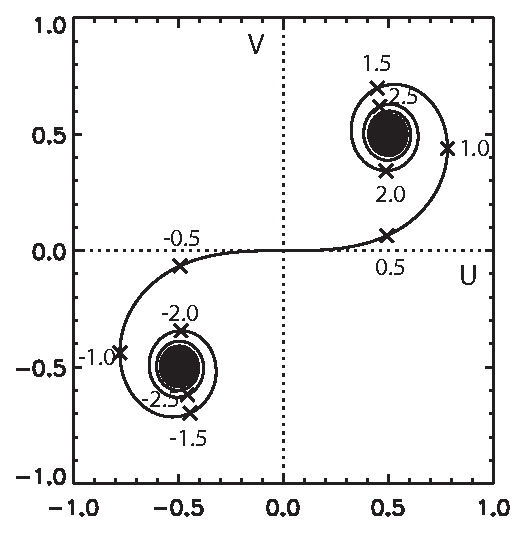
\includegraphics[width=0.7\textwidth]{cornu.eps}
  \caption{The Cornu Spiral showing the behaviour of the Fresnel integrals
$U(\xi)$ and $V(\xi)$. }
  \label{fig:cornu}
\end{figure}

The expression above is quite general. Let us here concentrate on the 
Fresnel diffraction pattern for an incoming plane wave that falls 
perpendicularly on the aperture, so $\psi_{\cal Q}$ is constant over the
aperture. Let us also confine ourselves to a rectangular aperture, with edges
along the $x'$ and $y'$ directions. Then the two integrals have limits that 
are independent of each other and that can be expressed in the form
$S(s_{max})-S(s_{min})$ and $S(t_{max})-S(t_{min})$ so

\be
\psi_{\cal P}={-i\over 2}[S(s_{max})-S(s_{min})][S(t_{max})-S(t_{min})]\psi_{\cal Q}e^{ikz}\equiv{-i\over 2}\Delta S_s\Delta S_t\psi_{\cal Q}e^{ikz},
\label{eq:fresnel}
\ee
where the arguments are the limits of integration and where
\[
S(\xi)\equiv\int_0^\xi e^{i\pi s^2/2}ds\equiv U(\xi)+iV(\xi)
\]
with
\bua
U(\xi)&=&\int_0^\xi ds\,\cos({\pi s^2/2}) \\
V(\xi)&=&\int_0^\xi ds\,\sin({\pi s^2/2})
\eua
\noindent
The real functions $U(\xi)$ and $V(\xi)$ are known as the {\it Fresnel integrals}.

The Fresnel integrals can be exhibited graphically using the {\it Cornu spiral},
which is a graph of the parametric equation $[U(\xi),V(\xi)]$, or equivalently
a graph of $S(\xi)=U(\xi)+iV(\xi)$ in the complex plane. 

The simplest illustration is the totally unobscured, plane wavefront. In this
case the limits of both integrations extend from $-\infty$ to $+\infty$, which
as is seen from figure~\ref{fig:cornu} is an arrow of length $\sqrt{2}$ and 
phase
$\pi/4$. Therefore, $\psi_{\cal P}$ is equal to 
$(2^{1/2}e^{i\pi/4})^2({-i/2})\psi_{\cal Q}e^{ikz}=\psi_{\cal Q}e^{ikz}$, as we 
could have seen from solving the Helmholtz equation for a plane wave.

Still following Kip Thorne's lecture notes, we make the following points

\begin{itemize}
\item Considering the integral derived above it is clear that only those light paths that 
are within a few Fresnel lengths of the geometric-optics path of least distance contribute
to the wave field at the point $\cal{Q}$.
\item Reltated to this, when computing the diffraction pattern from a more complicated 
aperture it is only necessary to perform the integral in the immediate vicinity of the 
geometric-optics ray. 
\item Finally, when integrating over the whole area of the wave front at $\cal{Q}$, we sum 
contributions with increasingly large phase differences that add up in such a way that the 
total has a net extra phase of $\pi/2$, relative the geometric optics ray. This phase factor
cancels exactly the prefactor $-i$ in the Fresnel-Kirchhoff integral.
\end{itemize}

\section{Lunar occultation of a radio source}

The next simplest case of Fresnel diffraction is the pattern formed by a straight 
edge. Let us take the example of a quasar's radio waves being occulted by the 
moon.
Treating the lunar limb as a straight edge, the radio source will create
a changing diffraction pattern as it passes behind the moon, and this pattern
can be measured by a radio telescope on the earth. Orient the coordinates
such that the moons edge is along the $y'$ (or $t$) direction. Then we have
$\Delta S_t\equiv S(t_{max})-S(t_{min})=\sqrt{2i}$ is constant, and 
$\Delta S_s\equiv S(s_{max})-(s_{min})$ is described by the Cornu spiral: long
before the occultation, $\Delta S_s$ is given by the arrow from $(-{1/2},-{1/2})$
to $({1/2},{1/2})$, {\it i.e.} $\Delta S_s=\sqrt{2i}$, and the observed amplitude
is $\psi_{\cal{Q}}e^{ilks}$. When the moon begins to occult the radio source, the
upper bound on the Fresnel integral begins to diminish from $s_{max}=+\infty$, 
and the complex vector on the Cornu spiral begin to oscillate in length and 
phase. The observed flux will also oscillate, more and more strongly as as 
geometric occultation is approached. At the point of geometric occultation, the
complex vector extends from $(-{1/2},-{1/2})$ to $(0,0)$ and so the observed
wave amplitude is one half the occulted value and the intensity is one fourth. 
As the occultation proceeds, the length of the complex vector and thus the 
observed flux will decrease monotonically to zero, while the phase continues to
oscillate.

Historically, diffraction of a radio source's waves by the moon led to the 
discovery of quasars. 

\section{Circular Apertures}

The diffraction pattern for a plane wave can be thought of as formed by waves 
that derive from a patch a few Fresnel lengths in size. This point can be 
driven home by reanalyzing the unobstructed wave front in circular polar
coordinates.

Consider a plane wave incident on an aperture $\cal{Q}$ that is infinitely 
large, and define 
$\rho\equiv{\labs{\bf x'}\labs/r_F}=\sqrt{{1\over 2}(s^2+t^2)}$. Then the 
phase factor in equation~\ref{eq:fresnel} is $\Delta\phi=\pi\rho^2$ and the
observed wave will thus be given by
\bua
\psi_{\cal{P}}&=&-i\int_0^\rho 2\pi\rho d\rho\,e^{i\pi\rho^2}\psi_{\cal{Q}}e^{ikz}\\
              &=&(1-e^{i\pi\rho^2})\psi_{\cal{Q}}e^{ikz}.
\eua
This integral does not converge as $\rho\rightarrow\infty$! Why is that? Add 
up the contributions to $\psi_{\cal{P}}$ from each annular ring as one integrates
outward from $\rho=0$; when one has integrated out to a radius of $r_F$, {\it i.e}
$\rho=1$, the contribution to the observed wave is $\psi_{\cal{P}}=2\psi_{\cal{Q}}$,
in phase with the incident wave. But, when the integration has been extended
to $\sqrt{2}r_F$, $\rho=\sqrt{2}$, $\psi_{\cal{P}}=0$. And as $\rho$ increases
the integral will continue to oscillate. 

Of course, we have already proven that this integral converges. Let us analyze 
what is going on by by splitting up the aperture $\cal{Q}$ into concentric
annular rings, known as {\it Fresnel half-period zones}, of radius $\sqrt{n}r_F$,
where $n=1,2,3,\ldots$. The odd numbered rings cancel out the contribution from
the even number rings. However, the thickness of these rings decreases as 
$1/\sqrt{n}$, and eventually one must allow for the fact that the incoming wave
is not exactly planar, or equivalently that the wave's distant source has 
finite size. The finite size causes the different pieces of the source to have 
their Fresnel rings centered at slightly different points in the aperture plane,
causing the computation of $\psi_{\cal{P}}$ to begin averaging over rings, and 
the intensity asymptotes to $\labs\psi_{\cal{Q}}\rabs^2$.

Why have we then chosen such a strange way of decomposing a plane wave front? 
Because it allows for a particularly striking experimental verification of the
theory of diffraction propounded here. Suppose one fabricates an aperture 
(a {\it zone plate}) in which, for a chosen observation point $\cal{P}$ on the 
optic axis, alternate half-period zones are obscured. Then the wave 
observed at $\cal{P}$ will be the linear sum of several diameters, and the sum
should be larger than $\psi_{\cal{Q}}$. This strong amplification is confined to
our chosen spot on the optic axis; most everywhere else the field's intensity
is reduced, thereby conserving energy. 
Thus, the zone plate behaves like a lens. 
The lens' focal length is $f={kA/2\pi^2}$, where A (typically chose to be a 
few mm$^2$ for a table top experiment) is the area of the first half-period 
zone. An interesting historical side note is that Poisson predicted this spot
as a consequence of Fresnel's theory of light, and was planning to use it
as an argument to disprove the theory. However, it was quickly demonstrated 
that the bright spot actually existed!

Zone plates are only good lenses when the radiation is monochromatic, since
the focal length is wavelength-dependent $f\propto \lambda^{-1}$. Further, they
have 
the interesting property that they posses secondary foci, where the fields from
$3,5,7,\ldots$ contiguous zones add up coherently.

\section{Seeing in the atmosphere}

\subsection{A simple model (with exercises)} \label{sec:seeing-model}

Stars viewed through the atmosphere appear to have angular diameters of 
order an arc second and to exhibit large amplitude fluctuations of flux with
characteristic frequencies that can be as high as 100~Hz. Both of these 
phenomena are a consequence of irregular variations in the refractive
index of the atmosphere. A simple model of this effect consists of a thin
phase-changing screen, about a km above the ground, on which the rms phase
variation is $\Delta\phi\gtrsim 1$ and the characteristic spatial scale on 
which the scale changes by $\sim\Delta\phi$ is $a$.

It is straightforward to show that rays will be irregularly deflected through
a scattering angle $\Delta\theta\sim({\lambda/a})\Delta\phi$. Strong 
intensity variations require that several rays deriving from points on the 
the screen separated by more than $a$, combine at each point on the ground.
These rays combine to create a diffraction pattern on the ground with
scale $b$. 

It is possible to show that the Fresnel length in the screen is 
$\sim\sqrt{ab}$. The time variation in the observed intensity arises because 
winds in the upper atmosphere with speeds $u\sim 30$~m$\,$s$^{-1}$ blow 
the irregularities and the diffraction pattern past the observer. The 
information given above is sufficient to estimate the Fresnel length $r_{F}$, 
the atmospheric fluctuation scale size $a$, and the rms phase variation 
$\Delta\phi$.

\subsection{Effects of the atomsphere (including better model)}

The two major effects of the Earth's atmosphere are {\it atmospheric
  refraction} and distorted wavefronts (or {\it seeing}) due to
refraction in a turbulent atmosphere.

We can approximate the atmosphere as a series of plane-parallel
plates, and the surface as an infinite plane. A ray incindent at angle
$\alpha$ refracts at each of the interfaces, and will ultimately make
a new angle $\alpha+\Delta\alpha$ with the surface: thus, refraction
shifts the apparent position of the source towards the zenith. The
atmosphere consists of a very large number of thin layers and the
total effect of refraction is to curve the path of the incident
ray. In this limit Fermat's principle and the plane-parallel model
gives 
\[
\Delta\alpha=R_0\tan{\alpha}={n^2-1\over 2n^2}\tan{\alpha}\approx
(n-1)\tan{\alpha}
\]
where $n$ is the index of refraction at the surface. The quantity
$(n-1)\times 10^6$ is the {\it refractivity}. Since the index is a
function of wavelength rays of different colors are refracted at
different angles, and at large zenith distances images are actually
very low resolution spectra --- with the blue image shifted more
towards the zenith than red.

\begin{figure}[h]
  \centering
	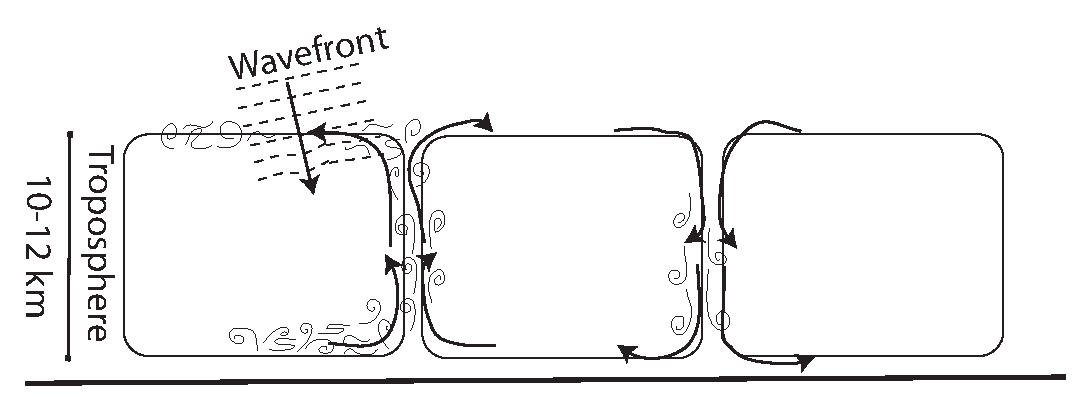
\includegraphics[width=0.9\textwidth]{seeing_global.eps}
  \caption{Sketch of atmospheric circulation in the troposphere and
    the effects it has on incoming wavefronts. Locally heated air near
    the ground will become boyant and rise, resulting in a convective
    flow as cool air flows to fill its place. Turbulence is enhanced
    at the boundaries of convection cells.}
  \label{fig:seeing_global}
\end{figure}

In a perfectly serene and quiet atmosphere, then density and index of
refraction of air will depend only on altitude, and every point at the
same height will have the same index. In the real atmosphere solar
heating drives convective cells in the lowest layer of the atmosphere,
a region some 10--12~km thick called the {\it troposphere}. One mass
of air can become slightly hotter and more bouyant than its neighbors
and therefore rise. Another mass moves horizontally to take its place;
cold air from above drops down to make room for the rising mass and
completes the circulation around a cell. Many cells are established,
and the air, especially at the boundaries of the flow, tends to break
up into turbulent eddies of different density and temperature. 

A wavefront from a distant star passing through the atmosphere arrives
as a plane, but different parts will encounter slightly different
patterns in the index of refraction. Each ray will traverse slightly
different optical path, and the wavefront will no longer be a
plane. Since the turbulent eddies at each altitude move at the local
wind speed, the distortion in the wavefront changes very quickly.

\begin{figure}[h]
  \centering
	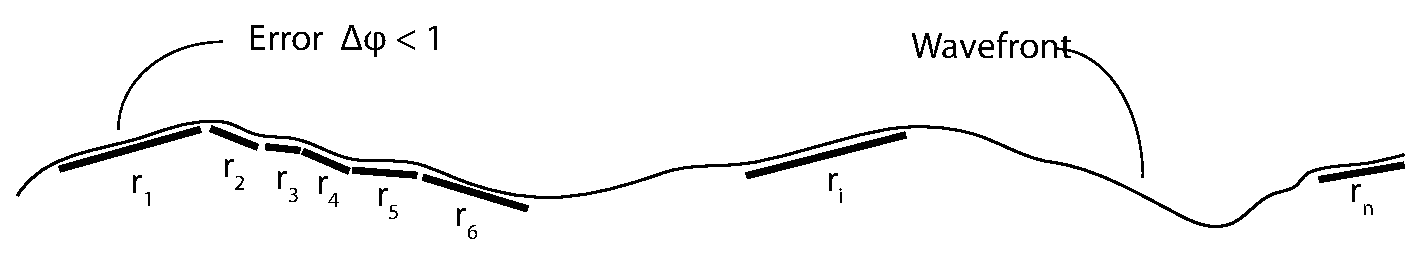
\includegraphics[width=0.9\textwidth]{wavefront_rn.eps}
  \caption{Quantifying the wavefront is done by fitting the wavefront
  with straight segments along which the difference between vertical
  $z$ direction between the fit and the wavefront is less than
  $\lambda/2\pi$ (equivalent to changes in phase $\Delta\phi<1$). The
  length of a segment $r_i$ is called the coherence length and the
  average of all segments is the coherence length of the wavefront.}
  \label{fig:wavefront_rn}
\end{figure}

We can quantify this wavefront distortion. Consider first a
one-dimensional model, start at one end of the wavefront and fit a
straight line to a segment of the front. How long can this segment be
before the fit becomes ``poor''? We need a criterion for judging the
goodness of fit, and we choose the root mean square (RMS) difference in the
vertical $z$ direction between the front and the fit. If this quantity
becomes greater than $\lambda/2\pi n$, then fit is poor. This is
equivalent that the RMS deviation of phase $\phi$ is less than one
radian. The maximum length that can be fit is $r_1$, called the
coherence length of the first segment. Moves along the front
fitting successive segments of ``good fit'' $r_i$. The statistical
mean of all the $r_i$ values is $r_{\rm avg}$ the {\it coherence
  length of the wavefront}. Each segment has a different slope, so
each will propagate in a slightly different direction, and each will
focus at a different spot in the image plane of a telescope. The
shorter the coherence length, the more {\it speckles} in the image.

Extending to two dimensions: select a random point on a
two-dimensional wavefront and ask how large a 2D patch of the front we
can expect to be choherent. The answer is called {\it Fried's
  parameter} $r_{0\lambda}$, the expected diameter over which the RMS
optical phase distortion is 1~radian.

\subsection{Real time atmospheric compensation}

Arguments of the sort given above (though with a somewhat more sophisticated
model of atmospheric turbulence) can be used to derive the maximum diameter
of a telescope before it becomes seriously affected by {\it seeing}, given
by Fried's coherence length 
\[
r_0\approx 0.114\left({\lambda\cos z\over 550}\right)^{0.6}~{\rm m}
\]
where $\lambda$ is the observing wavelength in nm and $z$ is the zenith 
angle. Fried's coherence length, $r_0$ is the distance over which the 
phase difference is one radian, and plays the same role as $a$ in the simpler
model above. In particular, the full width at half maximum of the
seeing disk is given by 
\[
\theta\approx 0.2{\lambda[\mu\mathrm{m}]\over r_{0\lambda}[\mathrm{m}]}
\]
If the diameter of a telescope, $D$, is larger than $r_{0\lambda}$,
then this expression gives the image size. If $D<r_{0\lambda}$ the
telescope is diffraction limited. Values for $r_0$ vary from a few
centimeters to 15 or 20~cm (which is excellent seeing).

Short of placing telescopes in space above the atmosphere, one alternative is
to correct the distortions introduced by atmospheric turbulence by the use
of adaptive optics. In such systems, one or more of the optical components
can be changed rapidly in such a manner that the undesired distortions
in the light beam are reduced or eliminated. 

The efficiency of an adaptive optics system is measured by the 
{\it Strehl ratio.} This quantity is the ratio of the intensity at the center
of the corrected image to that at the center of ta perfect diffraction 
limited image of the same source. The {\it normalized Strehl ratio} is the 
Strehl ratio of the corrected image divided by that for the uncorrected 
ratio. Strehl ratios of up to $0.6$ are currently being achieved and one may 
reach $0.8$ in the near future.

Note that a weakness of adaptive optics is that in the visual and near 
infrared, the correction only extends over a very small area (the 
{\it isoplanatic patch}). 

\begin{figure}[h]
  \centering
	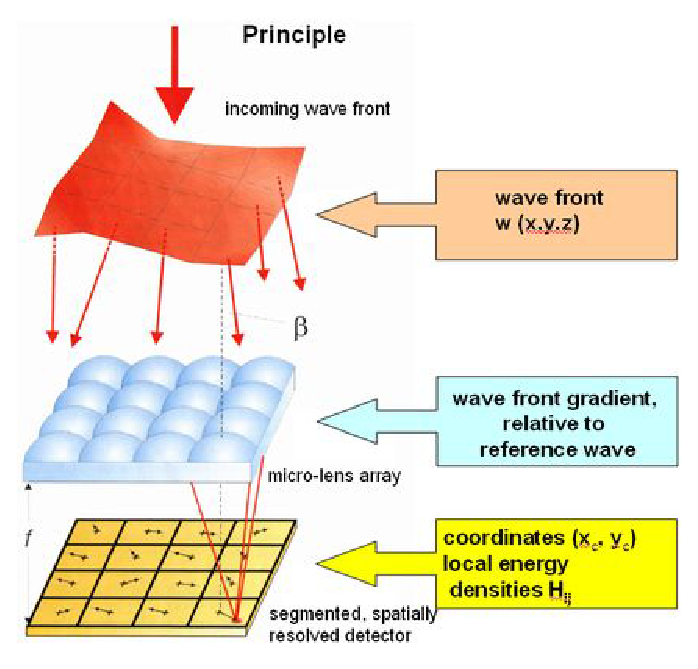
\includegraphics{shack-hartmann.eps}
  \caption{Prinicple of the Shack-Hartmann sensor. (figure from {\it
Institut f\"ur Photoniche Technologien e. V.)}}
  \label{fig:shack-hartmann}
\end{figure}

Note also that there is some confusion in the literature between terms 
adaptive optics and active optics. We will consider adaptive optics to
be those characterised by a fast closed-loop system, and active optics 
a more slowly operating open- or closed-loop system. The division is made
at at a response time of a few seconds. Thus, the tracking of a star by 
the telescope can be considered an active optics system that is open-loop 
if no guiding is used, and closed-loop if guiding is used. Large thin mirror
optical systems may suffer distortions due to buffeting by wind at a 
frequency of $0.1$~Hz or so; they may also distort under gravitational loading
or thermal stresses. Correction of these sorts of effects also goes under
the heading active optics. 

\begin{figure}[h]
	\centering
	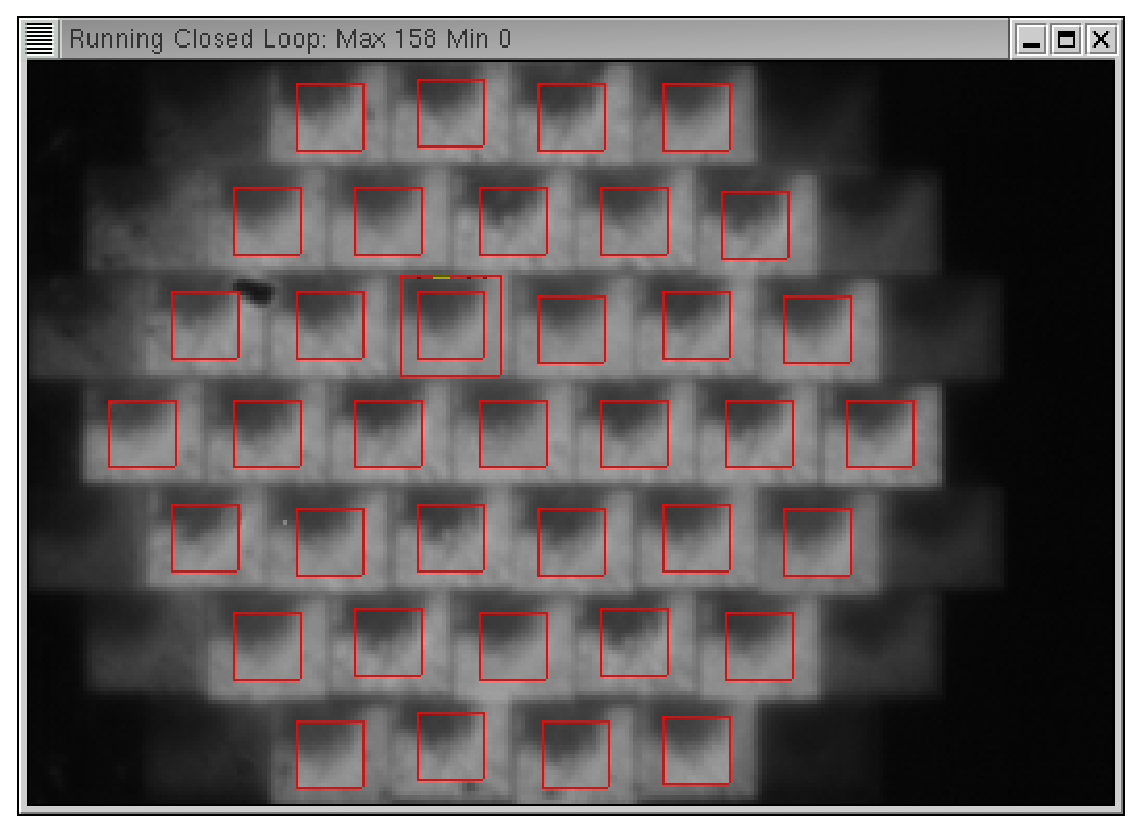
\includegraphics[width=0.9\textwidth]{AO_live_display.eps}
  \caption{The multiple images of the Shack-Hartmann micro lenses as seen 
in the Swedish 1~meter Solar Telescope.}
  \label{fig:ao_live_display}
\end{figure}

An atmospheric compensation system contains three main components, a
sampling system, a wave front sensor, and a correcting system.

\noindent
{\it Sampling systems.} The sampling system provides the sensor with the 
distorted wave front or a simulacrum thereof. A beam splitter is commonly used.
This is a partially reflecting mirror that typically diverts about 
$10\%$ of the radiation to the sensor, while allowing the remaining $90\%$
 to continue on to form the image. 

In night time astronomy even the loss of $10\%$ of the light is to be 
regretted. Many adaptive systems therefore use a guide star rather than the
object of interest to measure the wave front. This becomes especially important
when the object to be imaged is a large extended object, since sensors 
generally must be used on point or near point images (or at least images with
sharp gradients, see figure~\ref{fig:ao_live_display}). The guide star
must be very near in the sky to the object of interest or its wave front will
have gone through different atmospheric distortion. The isoplanatic patch
is defined by the distance over which the Strehl ratio improvement due to
the adaptive optics halves. In the visible it is typically of order
15~arcsec. The size of this patch scales as $\lambda^{1.2}$, so it is larger
in the infrared, reaching typically 80~arcsec at $2.2$~$\mu$m.

The small size of the isoplanatic patch means that few objects have suitable
guide stars; less than 1\% of the the sky can be covered using real stars
as guides. Recently therefore, artificial guide stars have been produced. 
This is done by using lasers pointed skywards. The laser is tuned to one of 
the sodium (Na) D~line frequencies and excites the free sodium atoms in the
atmosphere at a height of about 90~km. The glowing atoms appear as star-like
patches that can be placed as near in the sky to the object of interest as
required. Guide stars at lower altitudes and at other wavelengths can be 
produced through back scattering by air molecules of a laser beam. 
Two difficulties with this technique are the {\it cone problem} due the
geometry of the laser setup compared with the telescope and the fact that
the laser light also must pass {\it up} through the atmosphere and therefore
the guide star moves with respect to the object. Use of real stars to separately
compensate tip-tilt, and the use of two or several guide stars can eliminate
some or parts of this problem.

\noindent
{\it Wave front sensing.} The wave front sensor detects the residual and 
changing distortions in the wave front provided by the sampler after 
reflection from the correcting mirror. The Shack-Hartmann sensor is a two
dimensional array of small lenses (figure~\ref{fig:shack-hartmann}). Each
lens produces an image that is sensed by an array detector. In the absence
of wave front distortions, each image will be centered on each detector.
Distortion will displace the images from the centers of the detectors, and
the degree of displacement and its direction is used to generate the error
signal. 

\noindent
{\it Wave front correction.} The correction of the wave front is achieved
by distorting a subsidiary mirror. Since the atmosphere changes on a time
scale of 10~ms or so, the sampling, sensing and correction have to occur in
1~ms or less. In the simplest systems only the tip and tilt of the wave
front introduced by the atmosphere is corrected. That is accomplished by 
suitably inclining a plane or segmented mirror placed in the light beam
from the telescope in the opposite direction. 

More sophisticated approaches provide better corrections; either just
of the relative displacements within the distorted wave front, or of both
displacement and fine scale tilt. Displacement correction typically uses
a thin mirror capable of being distorted by up to 100~piezo-electric or other
actuators placed underneath. The error signal from the sensor is used to
distort the mirror in the opposite manner to the distortions in the incoming
wave front. The reflected wave front is therefore almost flat.

Plans for future 50~m and 100~m telescopes include adaptive secondary or
tertiary mirrors up to 8~m in diameter, requiring up to $500\,000$ actuators
to compensate the atmospheric distortions of the wave front.

\section{Exercises}
\begin{enumerate}[labelindent=\parindent, align=left, leftmargin=!,
		series = questions]
	\item Why is $\Delta\phi\approx {k{\bf x'}^2\over 2z}$ in Eq.~\ref{eq:phase_difference}?
	\item Check that the transition to a double integral in Eq.~\ref{eq:exercise2-chapter7-eq}
		is correct.
	\item Derive a formula for the intensity diffraction pattern $F(x)$ of a slit with width
		$a$, as a
		function of distance $x$ from the center of the slit, in terms of Fresnel integrals. 
	\item Recreate figure~\ref{fig:cornu} using {\sc idl}. The following fragments of code might 
		be useful
\belowcaptionskip=-10pt
\begin{lstlisting}[caption=Useful code I]
function fresnel_cos,xi
;
fcos=fltarr(n_elements(xi))
for i=0,n_elements(xi)-1 do begin
	npt=10000
	s=findgen(npt)/npt*xi[i]
	fcos[i]=trapez(s,cos(!pi*s*s/2.))
endfor
return,fcos
;
end
\end{lstlisting}
and equivalent for {\tt fsin}, which both call the function
\belowcaptionskip=-10pt
\begin{lstlisting}[caption=Useful code II]
function trapez,x0,y0
;
n=n_elements(x0)
x=fltarr(n)+x0
y=fltarr(n)+y0
integrand=(y+shift(y,-1))*(shift(x,-1)-x)
return,total(integrand(0:n-2))*0.5
;
end
\end{lstlisting}
(I am sure that this integral can be done in a {\bf much} better way
using calls to the error function ${\rm
  erf}(x)={2\over\sqrt{\pi}}\int_0^xe^{-t^2}dt$!, but this will work.)
\item Using {\sc idl}  and the routines above, plot the one-dimensional intensity diffraction pattern
  $\labs\psi\rabs^2$ produced by a slit, $t(x)=1$ for $\rabs x\labs<
  {a/2}$ and $t(x)=0$ for $\labs x\rabs > {a/2}$, for the values
  ${r_F/a}=0.05, 0.5, 1, 2$.
\item Explain why the focal length of a zone plate is $f={kA/2\pi^2}$. 
\item An opaque, perfectly circular disk of diameter $D$ is placed perpendicular
	to an incoming plane wave. Show that, at distances $r$ such that $r_F\ll D$, the
	disk casts a rather sharp shadow, but at the precise center of the shadow there
	should be a bright spot. How bright?
\end{enumerate}
\begin{enumerate}[series=info, leftmargin=\parindent,
		listparindent=\parindent]
	\item[] Use Section~\ref{sec:seeing-model} to answer the questions below.
\end{enumerate}
\begin{enumerate}[resume* = questions]
\item Explain why $\Delta\theta\sim({\lambda/a})\Delta\phi$.
\item Show that the Fresnel length in the screen is $\sim\sqrt{ab}$. 
\item Use the information given above to estimate $r_F$, the atmospheric fluctuation
scale $a$, and the rms phase variation $\Delta\phi$.
\end{enumerate}
